% Edit the title below to update the display in My Documents
%\title{Project Report}
%
%%% Preamble
\documentclass[paper=a4, fontsize=11pt]{scrartcl}
\usepackage[T1]{fontenc}
\usepackage{fourier}

\usepackage[english]{babel}															% English language/hyphenation
\usepackage[protrusion=true,expansion=true]{microtype}	
\usepackage{amsmath,amsfonts,amsthm} % Math packages
\usepackage[pdftex]{graphicx}
\usepackage{caption}
\usepackage{url}
\usepackage[table,xcdraw]{xcolor}
\usepackage{flafter} 
\usepackage[section]{placeins}

\usepackage{hyperref}
\hypersetup{
    colorlinks=true,
    linkcolor=blue,
    filecolor=magenta,      
    urlcolor=cyan,
}


%%% Custom sectioning
\usepackage{sectsty}
\allsectionsfont{\centering \normalfont\scshape}


%%% Custom headers/footers (fancyhdr package)
\usepackage{fancyhdr}
\pagestyle{fancyplain}
\fancyhead{}											% No page header
\fancyfoot[L]{}											% Empty 
\fancyfoot[C]{}											% Empty
\fancyfoot[R]{\thepage}									% Pagenumbering
\renewcommand{\headrulewidth}{0pt}			% Remove header underlines
\renewcommand{\footrulewidth}{0pt}				% Remove footer underlines
\setlength{\headheight}{13.6pt}


%%% Equation and float numbering
\numberwithin{equation}{section}		% Equationnumbering: section.eq#
\numberwithin{figure}{section}			% Figurenumbering: section.fig#
\numberwithin{table}{section}				% Tablenumbering: section.tab#


%%% Maketitle metadata
\newcommand{\horrule}[1]{\rule{\linewidth}{#1}} 	% Horizontal rule

\title{
		%\vspace{-1in} 	
		\usefont{OT1}{bch}{b}{n}
		\normalfont \normalsize \textsc{Department of Computer Scienece} \\ [25pt]
		\horrule{0.5pt} \\[0.4cm]
		\huge Programming Project Computer Vision -- Report \\
		\horrule{2pt} \\[0.5cm]
}
\author{
		\normalfont 								\normalsize
        Kunis Daniel, Maier Florian, Rüba Simon\\[-3pt]		\normalsize
        \today
}
\date{}


%%% Begin document
\begin{document}
\maketitle
\section*{Preface}
This report presents our approach for solving typical problems in Visual Geometry and gained insights and observations. The code can be accessed \href{https://git.uibk.ac.at/csat8361/visualgeometry}{here}.

\section*{Objective}
Insert an artificially rendered object into a movie such that everything is geometrically consistent (we will not worry about correct shading, occluders in front of the inserted object etc.).

\section*{Camera internal calibration}
The code for camera calibration is located in the \emph{src/camera\_calibration.py}. Below we will thoroughly describe the chosen algorithm.\\\\In order to recover the camera matrix $P$:
\begin{itemize}
\item We used the \href{https://github.com/opencv/opencv/blob/master/samples/data/chessboard.png}{OpenCV's sampled chessboard image} as a sufficiently richly structured scene and took several photos of it that are located in the `resources/chessboard` folder of our project. The advantage of using a chessboard is that it establishes a new coordinate system within itself: we can address the internal corners of the chessboard like points where `(0, 0)` is the upper left internal corner. This significantly simplifies the problem of finding correspondences of points that we will use for finding $P$.
\item Now we consider each image one by one and find the coordinates of the corners of the chessboard using the \href{https://docs.opencv.org/2.4/modules/calib3d/doc/camera_calibration_and_3d_reconstruction.html#findchessboardcorners}{cv2.findChessboardCorners} function. After the image coordinates of the corners are retrieved we improve their accuracy using \href{https://docs.opencv.org/2.4/modules/imgproc/doc/feature_detection.html#cv2.cornerSubPix}{cv2.cornerSubPix}. After iterating over all images we have two arrays: `obj\_points` -- with object points in the calibration pattern coordinate space; and `img\_points` -- projections of calibration pattern points for each image.
\item Solve the correspondences for $P$ using the \href{https://docs.opencv.org/2.4/modules/calib3d/doc/camera_calibration_and_3d_reconstruction.html#cv2.calibrateCamera}{cv2.calibrateCamera} method. Under the hood it consists of 3 steps:
\begin{itemize}
\item \emph{Initialization}. Compute an initial value for the camera matrix using DLT. Assume that distortion coefficients are zero.
\item \emph{Initial estimation}. Estimate the initial camera pose as if the intrinsic parameters have been already known using \emph{cv2.solvePnP()}.
\item \emph{Iterative optimization}. Minimize the reprojection error using the Levenberg-Marquardt optimization algorithm.
\end{itemize}
The reprojection error is a geometric error and it is the mean value of squared distances between the observed projections img\_points (that were retrieved by the corner finding algorithm) and the projected (using \emph{cv2.projectPoints}) obj\_points.
\end{itemize}

The described method is alike the \emph{Gold Standard} algorithm described in \href{http://www.robots.ox.ac.uk/~vgg/hzbook/}{HZ} in 4.5 (p114).

\subsection*{Observation 1}
During our first iteration we used the \href{https://github.com/opencv/opencv/blob/master/samples/data/left01.jpg}{chessboard images provided by OpenCV} which are of size \emph{640x480}. After switching to images made by our camera without changing any of the parameters we saw an excessive rise in the error (from \emph{0.024} up to \emph{0.5}) even though the quality and number of input images was increased from \emph{13} up to \emph{262} and we were expecting an error decrease. The explanation of this rise was that our new images were much bigger -- \emph{3024x4032} -- and the \href{https://docs.opencv.org/2.4/modules/imgproc/doc/feature_detection.html#cv2.cornerSubPix}{cv2.cornerSubPix} function could not find the absolute minimum within the given boundaries (we specify \emph{winSize} which is half of the side length of the search window) since the search window became relatively smaller to overall image size. We solved it by resampling large input images that are bigger than \emph{1920x1080} using the \href{https://docs.opencv.org/2.4/modules/imgproc/doc/geometric_transformations.html#resize}{cv2.resize} using the \emph{INTER\_AREA} interpolation method which is considered best for downsampling. This greatly improved  the result -- reprojection error became \emph{0.141}.

\section*{Inserting static shape into 3D scene using calibration rig}
In the beginning, as a first iteration, we decided to insert a cube into a 3D scene using a calibration rig which greatly simplifies the objective since we can use the chessboard as the coordinate system and we can easily find the point correspondences.\\\\The implementation of this step can be found in \emph{src/drawing.py} and can be decomposed into these steps:
\begin{itemize}
\item Convert input video to image sequence.
\item Iterate over all images and for each find the corners of the chessboard using \href{https://docs.opencv.org/2.4/modules/calib3d/doc/camera_calibration_and_3d_reconstruction.html#findchessboardcorners}{cv2.findChessboardCorners}, calculate the pose of the chessboard using RANSAC algorithm (implmetned in the \href{https://docs.opencv.org/2.4/modules/calib3d/doc/camera_calibration_and_3d_reconstruction.html?highlight=solvepnpransac#solvepnpransac}{cv2.solvePnPRansac} function), project the 3D points of the cube (in chessboards' coordinate system) to the 2D image plane, draw the cube and save the image.
\item Convert the image sequence to a video.
\end{itemize}
We chose RANSAC because of it's robustness and resistance to outliers.

\subsection*{Observation 2}
Do not use a square chessboard pattern. It might sound obvious, but we did not think of it in the beginning. Using a symmetrical rig confuses the algorithm and corrupts camera calibration and can be revealed only during the drawing of the cube.

\begin{figure}[h!]
\centering
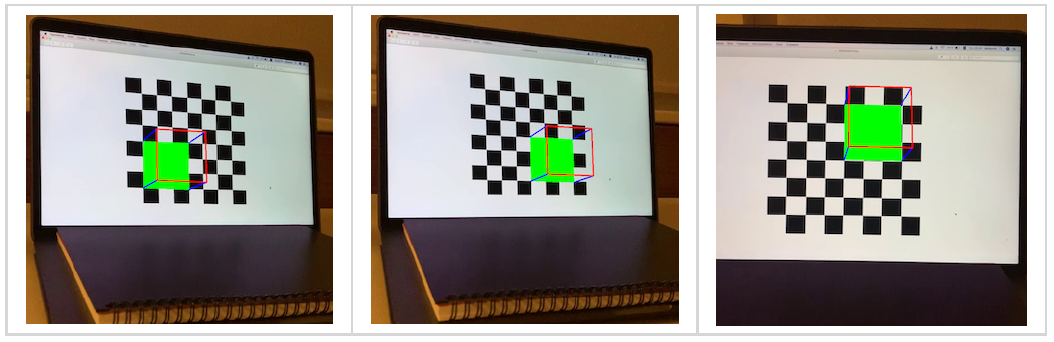
\includegraphics[width=1\textwidth]{img/staticShape}
\caption{Consider this image sequence. All of them are from the same video.}
\end{figure}

\section*{Getting the frames}
Our function \emph{video\_to\_frames} extracts frames from a video and saves them to a directory. We give the possiblity to skip frames (e.g. only take every 6th frame) in order to reduce the number of frames and to speed up the process. We ran the program twice: once with every frame and once with every 6th frame. The first option has a really long computation time. The second option is fast. The difference between the videos is hardly visible. We provide both videos.

\section*{Feature Matching and finding Keyframes}
The feature matching is done in our \emph{feature\_matching} function in \emph{point\_correspondences.py}.\\\\We tried keypoint detection with both SIFT and Harris Corner Detector. Since we got better results with SIFT (we got more points and they showed better results for scaling and rotating), we are using SIFT. However, we left our function that uses the Harris Corner Detector in the code (see: \emph{point\_correspondences.py} - \emph{get\_key\_points}).
\begin{figure}[h!]
\centering
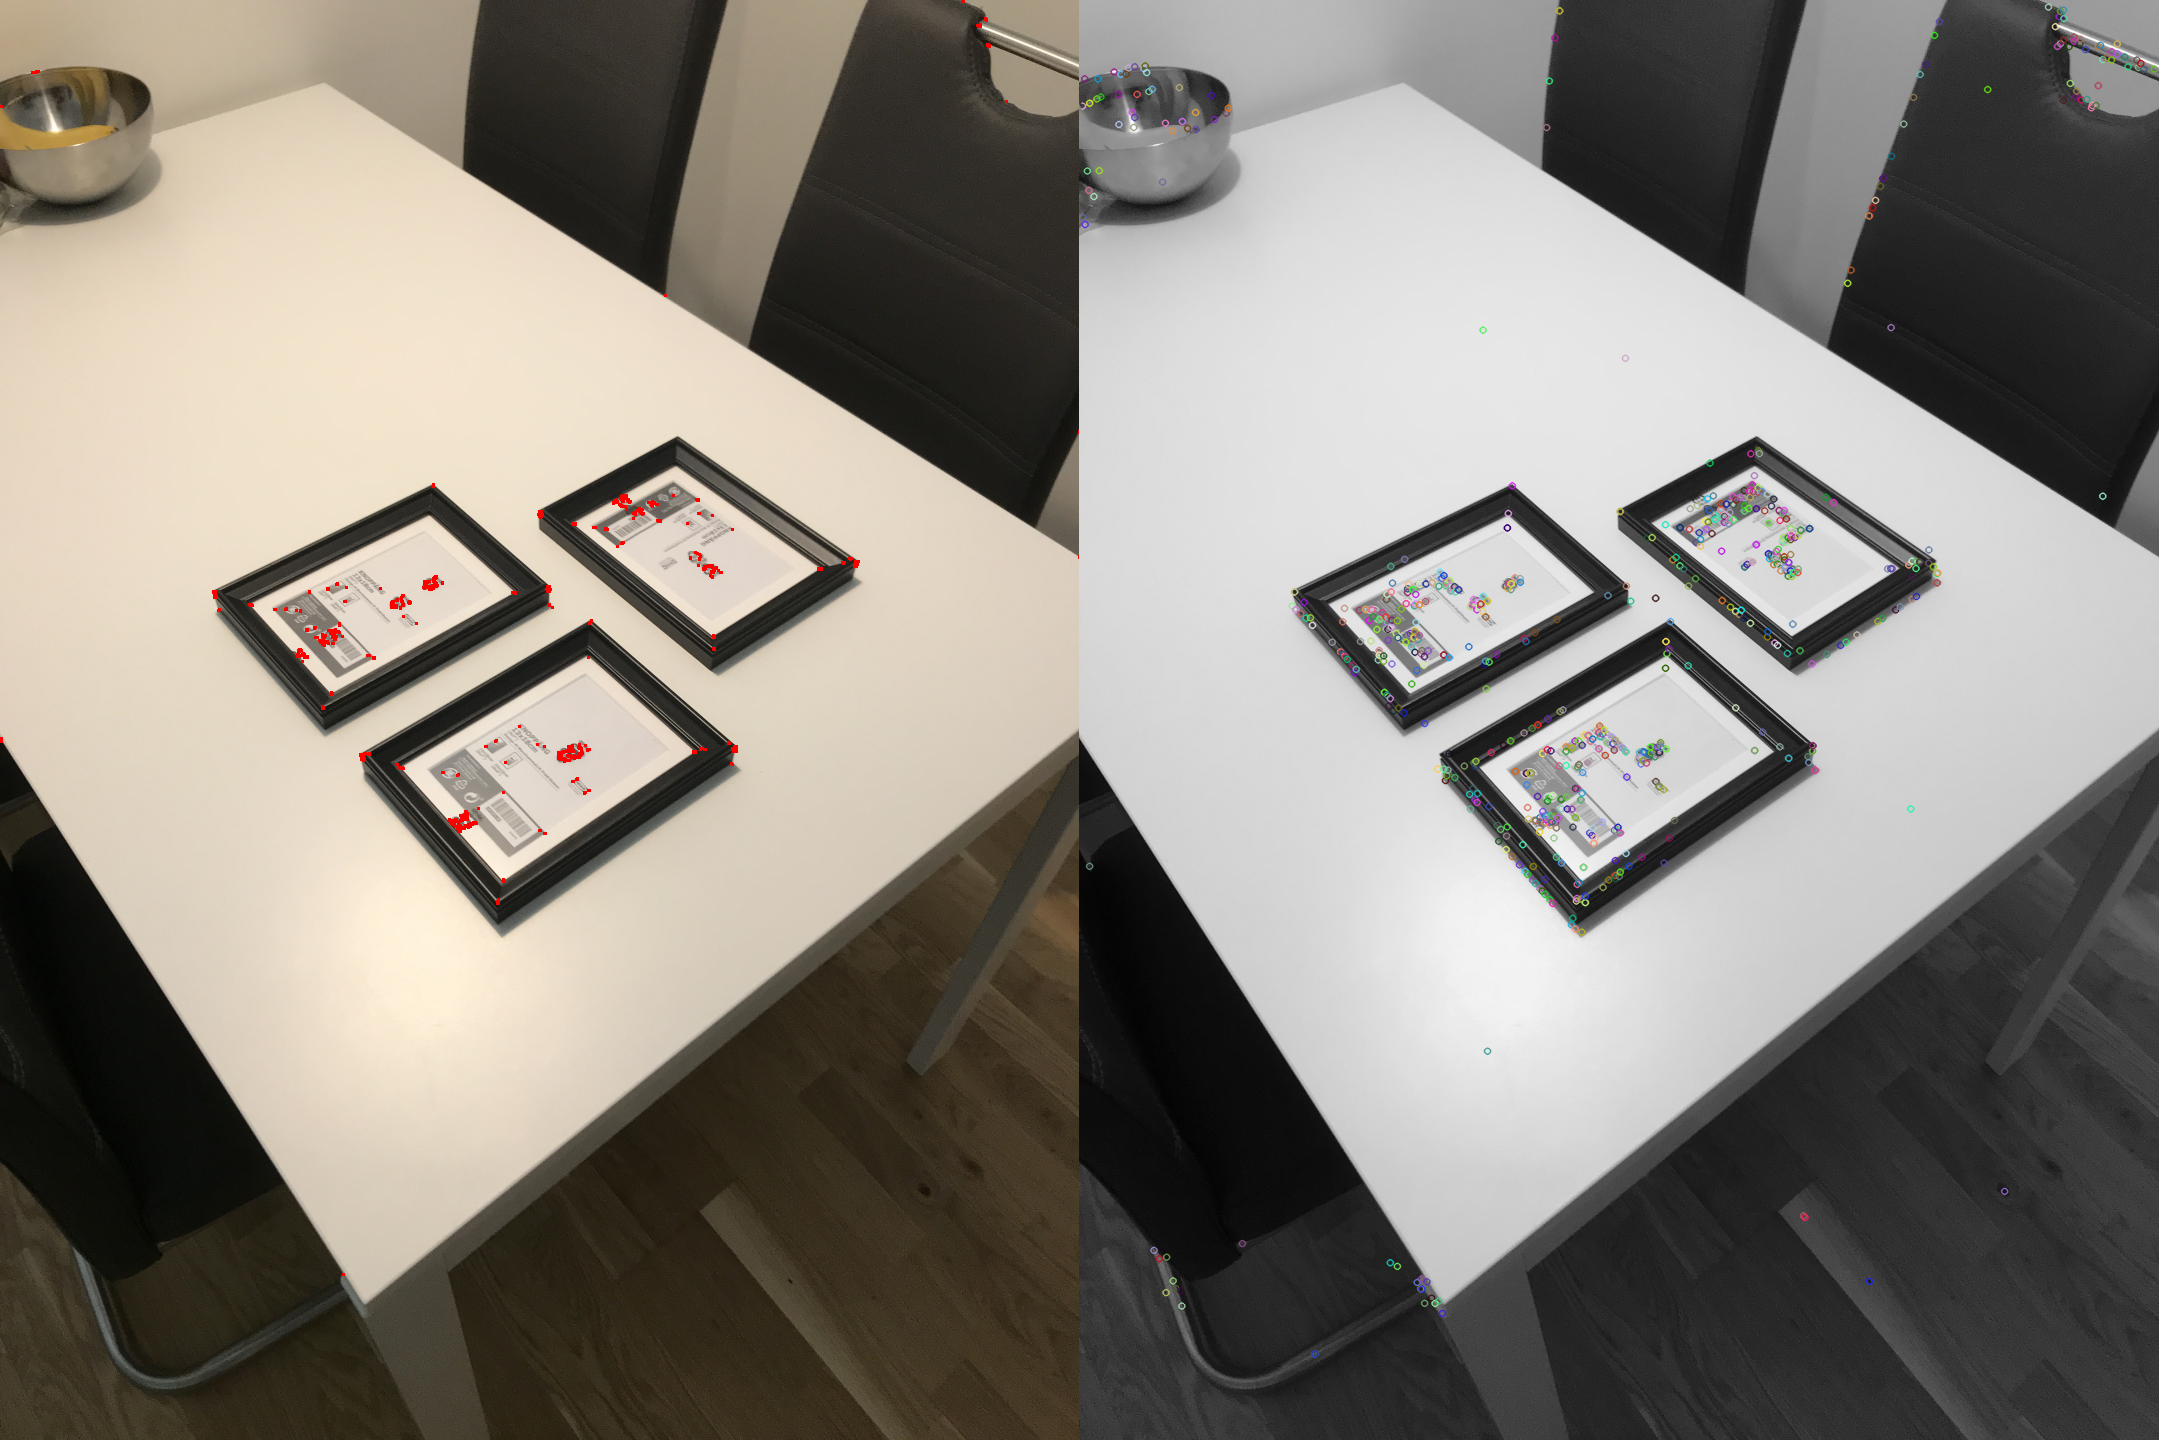
\includegraphics[width=1\textwidth]{img/hcdvssift}
\caption{Difference between Harris Corner Detector (Left) and SIFT (Right).}
\end{figure}
\\\textbf{Algorithm:}\\\\\underline{The desired output:} We want to find \emph{keypoints} that we can trace through all of the\emph{keyframes}. Moreover, we want all \emph{intermediate\_frame\_matches} (i.e. of non-keyframes), containing the matches between their frame points to the keypoints of the previous and following keyframe.
\begin{itemize}
\item Using the \emph{sift.detectAndCompute} function we find the keypoints of the first frame.
\item We save all sift points for the first keyframe by using a data structure from \emph{\href{https://jivp-eurasipjournals.springeropen.com/track/pdf/10.1186/s13640-017-0168-3}{A fast 3D scene reconstructing method using continuous video}}.
\item  In order to find keyframes, we iterate through all frames:
\begin{itemize}
\item detect sift points for the current frame
\item using the \emph{FLANN} algorithm we try to find 2 points in the current frame which are possible matches for a keypoint of the previous keyframe. Then we filter the results with Lowe's ratio test. The best result (i.e. the point which match the keypoint) must be less than 70\% than the distance of the second best.
\item Optional: draw the matches and save the image
\item Check if the current frame fulfills the requirements to be a keyframe. We decided to choose the requirements presented in \emph{\href{https://jivp-eurasipjournals.springeropen.com/track/pdf/10.1186/s13640-017-0168-3}{A fast 3D scene reconstructing method using continuous video}}, chapter 3.1, adjusted for our objective:
\begin{itemize}
\item The average feature distance in pixel must be more than ImageWidth/17.
\item Feature point matcches did not drop dramatically with respect to previous match.
\end{itemize}
\end{itemize}
\end{itemize}
\underline{The acutal output:} In our last run of our program we got 56 frames. 11 of them were keyframes (the following frames were keyframes: 0, 3, 9, 13, 16, 19, 27, 35, 41, 49, 55). The distribution of the keyframes looks very good.

\begin{figure}[h!]
\centering
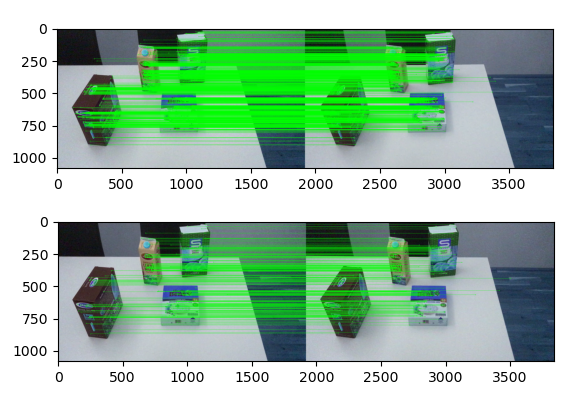
\includegraphics[width=1\textwidth]{img/matching}
\caption{Matching Keypoints. First Picture shows matching between frame 0 and frame 1. Second Picture shows matching between frame 9 and frame 10}
\end{figure}

\section*{Stereo Reconstruction}
After finding the keyframes and matching the keypoints, we want to compute the camera matrices for every frame. This is done in our \emph{stereo\_reconstruction} function.\\\\\textbf{Preparation:} We created a \emph{Camera} class where we can save the rotation \emph{R}, translation \emph{t} and projection matrix \emph{P}.\\\\For the initial reconstruction we used the algorithm presented in \href{http://www.robots.ox.ac.uk/~vgg/hzbook/}{HZ} (\emph{chapter 18.6}, \emph{algorithm 18.3}, "Extending the baseline"). We set our first keyframe as our origin (i.e. no rotation and translation). Using the previously calculated matches we calculate the camera of the last keyframe.\\Then we calculate the 3d points by triangulation. Having them, we calculate the cameras for all other keyframes by resectioning using the \emph{cv2.solvePnPRansac} function. At the end, we recover all intermediate cameras.

\section*{Drawing the cube}
At this time we have the cameras for all frames. Using a photo-editor (e.g. GIMP), we select 4 points in our first keyframe and the same 4 points in the last keyframe. By triangulating we then get 4 world points. We then hardcode the other 4 worldpoints, so it forms a cube.\\After that we iterate over all frames and by using the \emph{cv2.projectPoints} function, we get the 2d image points of the cube for every frame. By connecting all corners, we draw the cube. Every frame gets saved and at the end they get converted to a video.\\\\\textbf{Additional Information:} Since our final result was pretty good in our opinion, we decided that bundle adjustment is not needed.

\begin{figure}[h!]
\centering
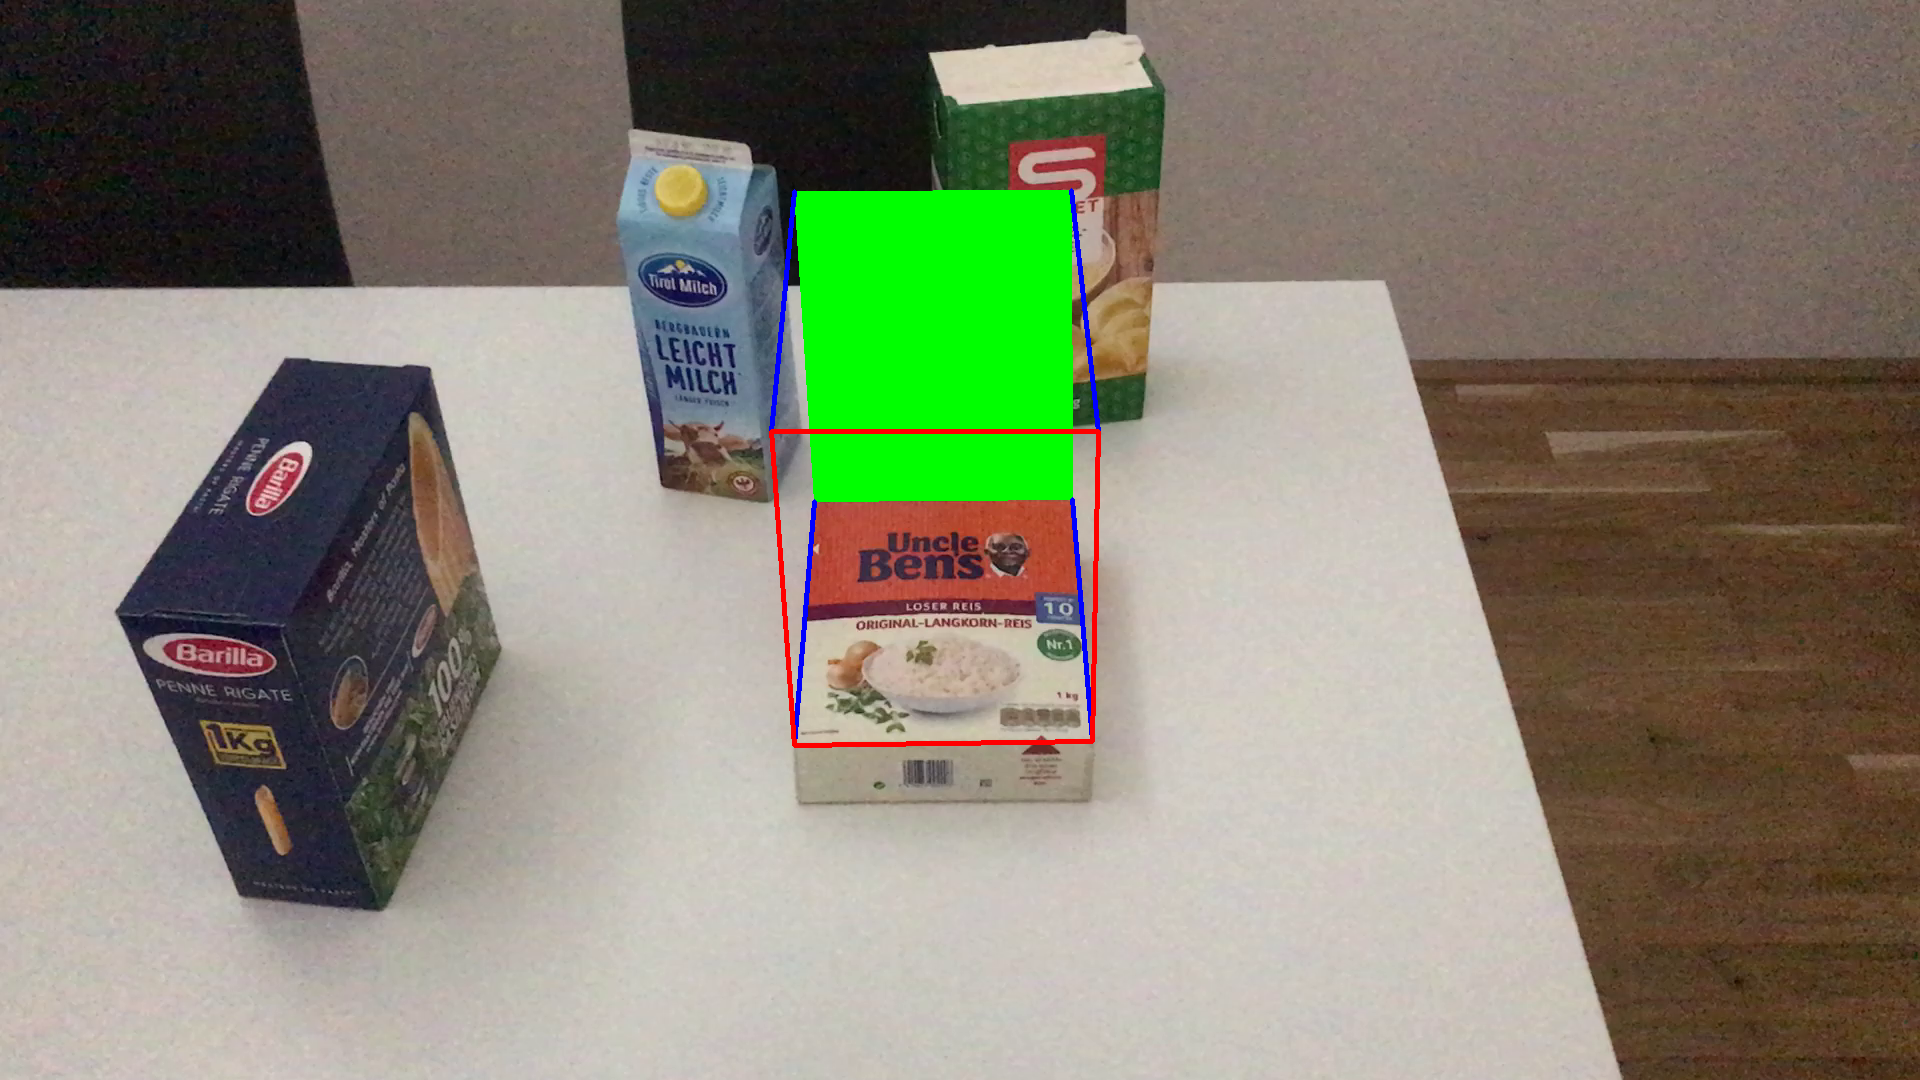
\includegraphics[width=1\textwidth]{img/firstframe}
\caption{Drawing of the cube. First frame (out of 56)}
\end{figure}

\begin{figure}[h!]
\centering
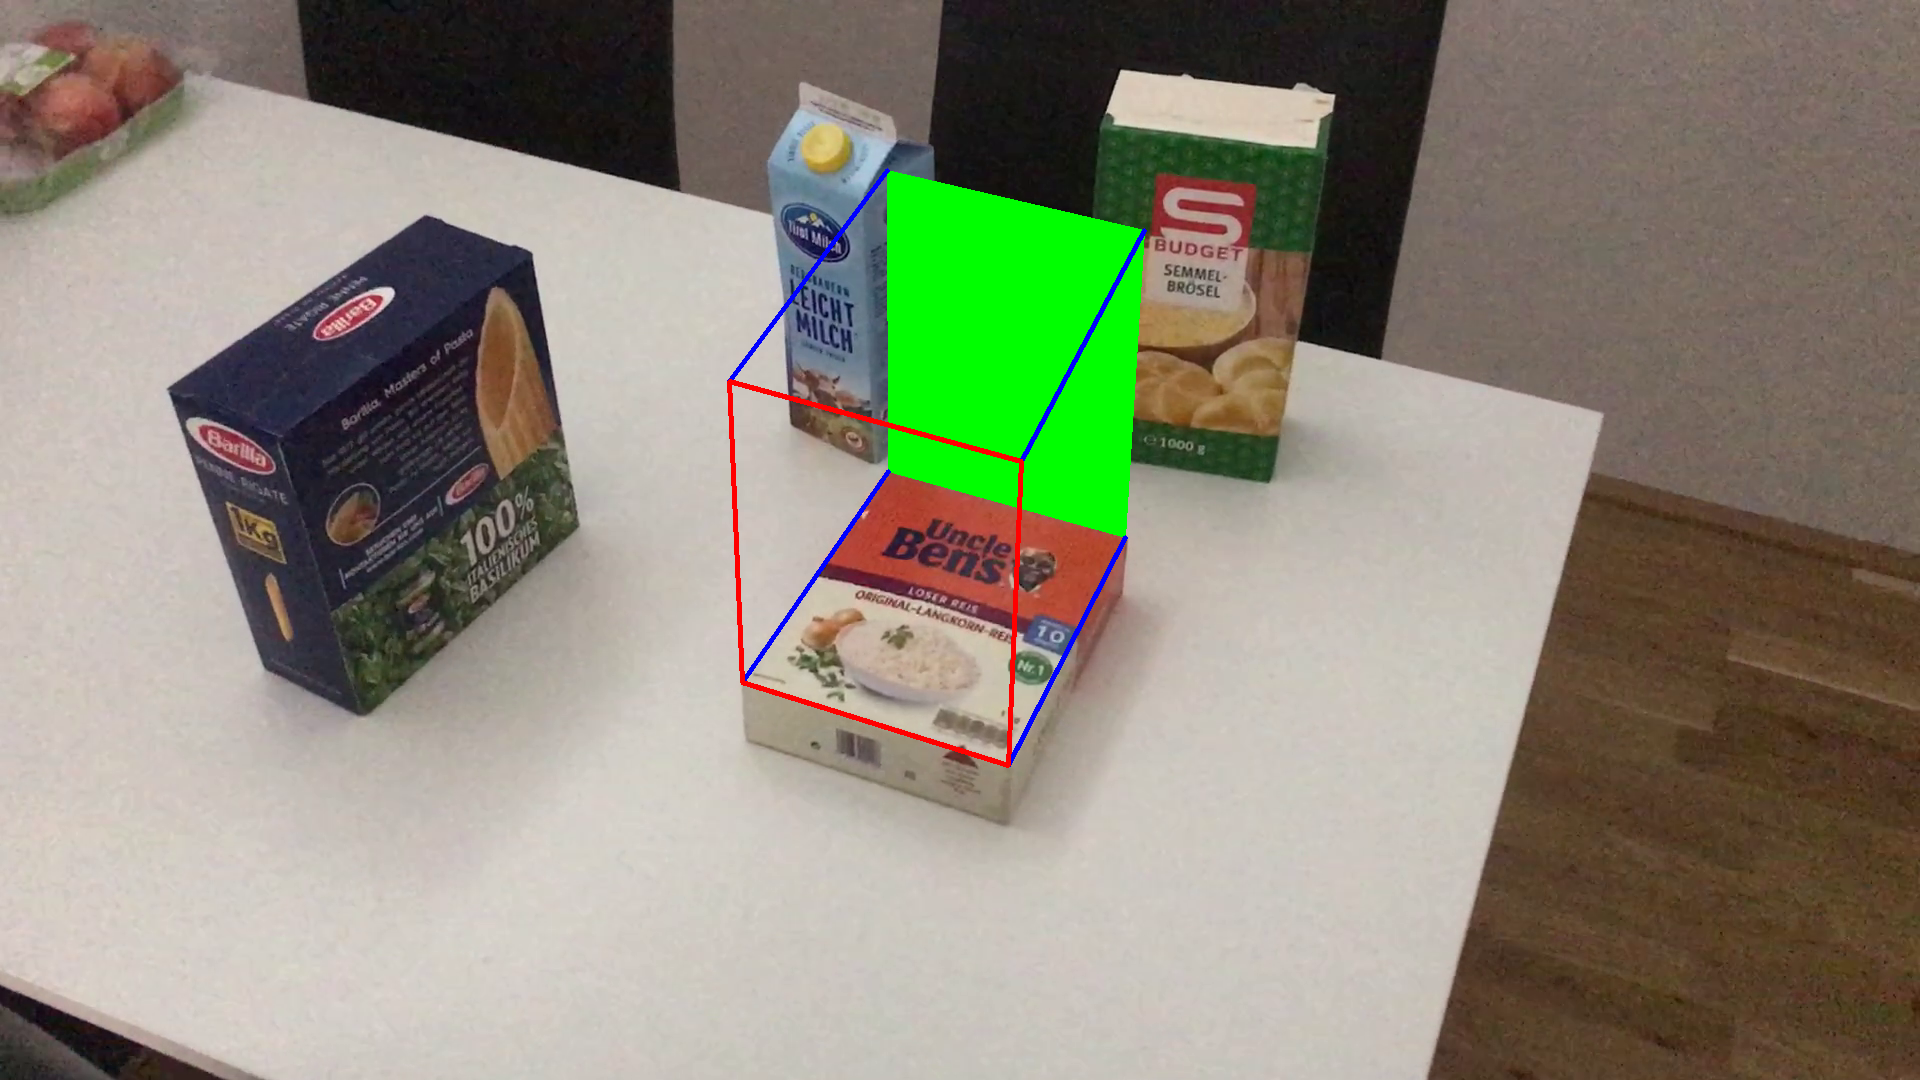
\includegraphics[width=1\textwidth]{img/frame28}
\caption{Drawing of the cube. Frame 28}
\end{figure}

\begin{figure}[h!]
\centering
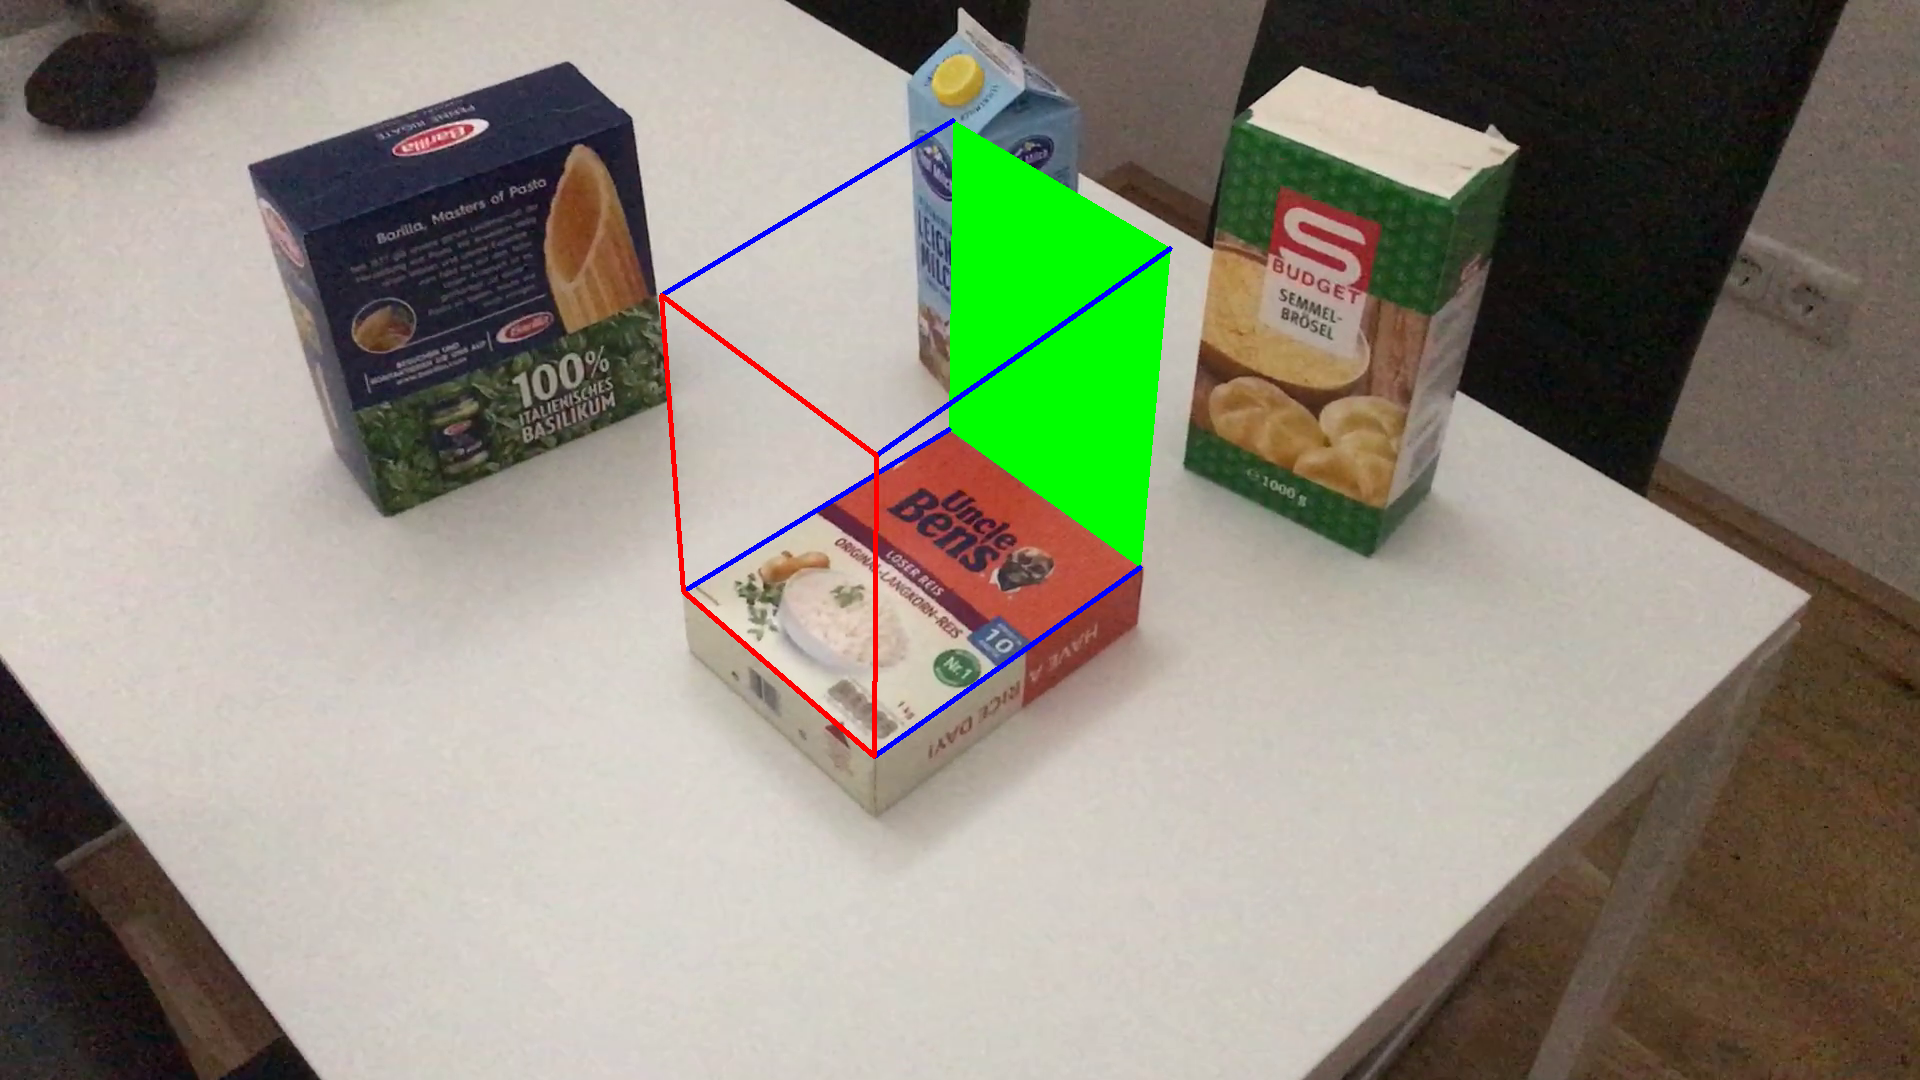
\includegraphics[width=1\textwidth]{img/lastframe}
\caption{Drawing of the cube. Last frame (out of 56)}
\end{figure}

\begin{figure}[h!]
\centering
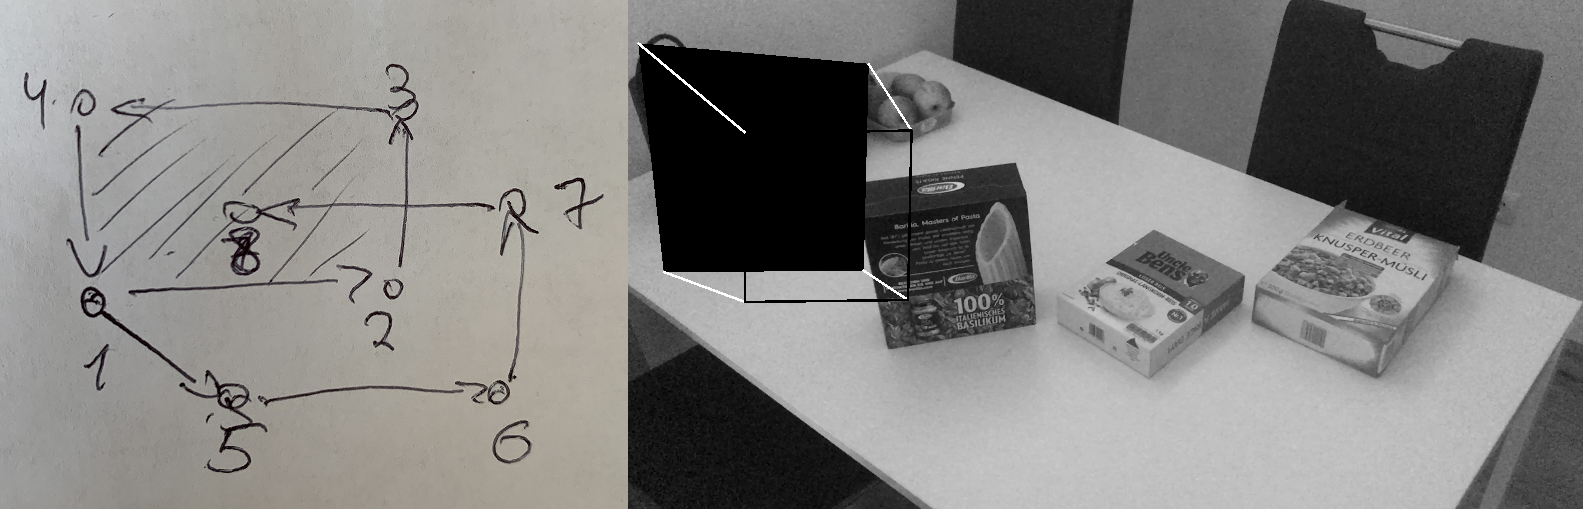
\includegraphics[width=1\textwidth]{img/tryingCube}
\caption{How we tried to fix our cube. Point 1 to 8 represent the order of our hardcoded cube}
\end{figure}

\section*{Contributions}
\begin{table}[!htbp]
\begin{tabular}{|l|ccc|}
\hline
{\color[HTML]{656565} }                        & {\color[HTML]{9B9B9B} Kunis Daniel}         & {\color[HTML]{9B9B9B} Maier Florian}                   & {\color[HTML]{9B9B9B} Rüba Simon} \\ \hline
{\color[HTML]{9B9B9B} Camera Calibration}      & \multicolumn{1}{c|}{}                       & \multicolumn{1}{c|}{50\% (1)}                          & 50\% (2)                          \\ \cline{2-4} 
{\color[HTML]{9B9B9B} Utils}                   & \multicolumn{1}{c|}{30\%}                   & \multicolumn{1}{c|}{30\%}                              & 40\%                              \\ \cline{2-4} 
{\color[HTML]{9B9B9B} Feature Matching}        & \multicolumn{1}{c|}{Main part ($\sim$75\%)} & \multicolumn{1}{c|}{SIFT and HCD (3), drawing matches} &                                   \\ \cline{2-4} 
{\color[HTML]{9B9B9B} Stereo Reconstruction}   & \multicolumn{1}{c|}{100\%}                  & \multicolumn{1}{c|}{}                                  &                                   \\ \cline{2-4} 
{\color[HTML]{9B9B9B} Drawing Functions}       & \multicolumn{1}{c|}{}                       & \multicolumn{1}{c|}{}                                  & 100\%                             \\ \cline{2-4} 
{\color[HTML]{9B9B9B} Drawing the actual cube (4)} & \multicolumn{3}{c|}{Pair programming (with screen share)}                                                                                \\ \cline{2-4} 
{\color[HTML]{9B9B9B} Refactoring}             & \multicolumn{1}{c|}{at half-time}           & \multicolumn{1}{c|}{}                                  & at the end                        \\ \cline{2-4} 
{\color[HTML]{9B9B9B} Report}                  & \multicolumn{1}{c|}{Camera Calibration, drawing on rig}     & \multicolumn{1}{c|}{everything else}                   &                                   \\ \hline
\end{tabular}
\end{table}\smallskip\noindent(1) with sample chessboard images from the internet to test the algorithm\\(2) with our photos of the chessboard (producing the actual results)\\(3) The Code of SIFT and Harris Corner Detector wasn't used, but it is still in the .py file.\\(4) Including hardcoding 4 worldpoints, triangulation of 4 points and orientate the cube.


%%% End document
\end{document}